%%%%%%%%%%%%%%%%%%%%%%%%%%%%%%%%%%%%%%%%%%%%%%%%%%%%%%%%%%
%%%%%%%%%%%%%%%%%%%%%%%%%%%%%%%%%%%%%%%%%%%%%%%%%%%%%%%%%%
%%%%%%%%%%%%%%%%%%%%%%%%%%%%%%%%%%%%%%%%%%%%%%%%%%%%%%%%%%
%%%%%%%%%%%%%%%%%%%%%%%%%%%%%%%%%%%%%%%%%%%%%%%%%%%%%%%%%%
\chapter{Rayleigh-B\'enard}

%%%%%%%%%%%%%%%%%%%%%%%%%%%%%%%%%%%%%%%%%%%%%%%%%%%%%%%%%%
%%%%%%%%%%%%%%%%%%%%%%%%%%%%%%%%%%%%%%%%%%%%%%%%%%%%%%%%%%
%%%%%%%%%%%%%%%%%%%%%%%%%%%%%%%%%%%%%%%%%%%%%%%%%%%%%%%%%%
\section{Physics}

We consider the resolution of the 2D Navier-Stokes equations coupled to the heat equation in a cavity of length $L$ and height $H$, with a hot bottom plate and cold top plate. Under certain circonstances, this setup is known to lead to the Rayleigh-B\'enard convection cell, which is illustrated in figure \ref{fig:rayleigh_convection}. The resulting system is driven by the following set of equations:

\begin{equation}
\label{eq:rayleigh}
\begin{split}
	\nabla \cdot \V{u} 						&= 0, \\
	\partial_t \V{u} + (\V{u} \cdot \nabla) \, \V{u} 	&= -\nabla p + \sqrt{\frac{\pr}{\ra}} \nabla^2 \V{u} + \theta \V{\hat{y}}, \\
	\partial_t \theta + (\V{u} \cdot \nabla) \, \theta 	&= \frac{1}{\sqrt{\pr \, \ra}} \nabla^2 \theta,
\end{split}
\end{equation}

where $\V{u}$, $p$ and $\theta$ are respectively the non-dimensional velocity, pressure, and temperature  of the fluid. The adimensional temperature $\theta$ is described in terms of the hot and cold reference temperatures, respectively denoted as $T_H$ and $T_C$: 

\begin{equation*}
	\theta = \frac{T - \hat{T}}{\Delta T}, \text{with } \hat{T} = \frac{T_H + T_C}{2} \text{ and } \Delta T = T_H - T_C.
\end{equation*}

The dynamics of the system (\ref{eq:rayleigh}) are controlled by two adimensional numbers. First, the Prandtl number $\pr$, which represents the ratio of the momentum diffusivity over the thermal diffusivity: 

\begin{equation*}
	\pr = \frac{\nu}{\kappa},
\end{equation*}

where $\nu$ is the kinematic viscosity and $\kappa$ the thermal diffusivity. Second, the Rayleigh number $\ra$, which compares the characteristic time scales for transport due to diffusion and convection:

\begin{equation*}
	\ra = \frac{g \alpha \Delta T H^3}{\kappa \nu},
\end{equation*}

with $g$ the magnitude of the acceleration of the gravity and $\alpha$ the thermal expansion coefficient. We also define the instantaneous Nusselt number, $\nus$, as the adimensionalized heat flux averaged over the hot wall:

\begin{equation}
\label{eq:nusselt}
	\nus (t) = - \int_{0}^{L} \partial_y \theta (x',y=0,t) dx'.
\end{equation}

The system (\ref{eq:rayleigh}) is completed by the following initial and boundary conditions:

\begin{equation}
\label{eq:rayleigh_bc}
\begin{split}
	\V{u}(x,y,0)	= 0 &\text{ and } \theta(x,y,0)	= 0, \\
	\V{u}(x=0,y,t)	= 0 &\text{ and } \V{u}(x=L,y,t) = 0, \\
	\V{u}(x,y=0,t)	= 0 &\text{ and } \V{u}(x,y=H,t) = 0, \\
	\theta(x,y=0,t) 	= \theta_H &\text{ and } \theta(x,y=H,t) = \theta_C, \\
	\partial_x \theta(x=0,y,t) = 0 &\text{ and } \partial_x \theta(x=L,y,t) = 0,
\end{split}
\end{equation}

In essence, the boundary conditions (\ref{eq:rayleigh_bc}) correspond to (i) a no-slip boundary conditions for the fluid on all boundaries, (ii) imposed hot and cold temperatures respectively on the bottom and top plate, and (iii) adiabatic boundary conditions on the lateral sides of the domain. Here, we choose $\theta_H = \frac{1}{2}$ and $\theta_C = -\frac{1}{2}$. A sketch of the configuration is presented in figure \ref{fig:rayleigh_sketch}.

%%%%%%%%%%%%
%%%%%%%%%%%%
\begin{figure}
\centering
%%%%%%%%%%%%%%
\def\xaxis{5}
\def\yaxis{5}
%%%%%%%%%%%%%%
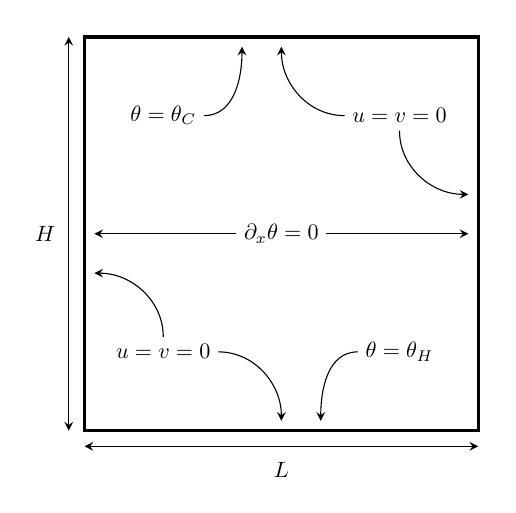
\begin{tikzpicture}[]

	%%% Domain
	\draw[black, very thick] (0,0) rectangle (\xaxis,\yaxis);
	
	%%% Dimensions
	\draw[stealth-stealth] (0,-0.2) -- (\xaxis,-0.2);
	\node[scale=0.8] at (0.5*\xaxis, -0.5) {$L$};
	\draw[stealth-stealth] (-0.2,0) -- (-0.2,\yaxis);
	\node[scale=0.8] at (-0.5,0.5*\yaxis) {$H$};
	
	%%% Velocity BC
	\node[scale=0.8] (bc_top_right) at (\xaxis-1,\yaxis-1) {$u=v=0$};
	\node (bc_top) at (0.5*\xaxis, \yaxis) {};
	\node (bc_right) at (\xaxis, 0.6*\yaxis) {};
	\draw[-stealth] (bc_top_right) to[out=180,in=-90] (bc_top);
	\draw[-stealth] (bc_top_right) to[out=-90,in=180] (bc_right);
	
	\node[scale=0.8] (bc_bot_left) at (1,1) {$u=v=0$};
	\node (bc_bot) at (0.5*\xaxis, 0) {};
	\node (bc_left) at (0, 0.4*\yaxis) {};
	\draw[-stealth] (bc_bot_left) to[out=0,in=90] (bc_bot);
	\draw[-stealth] (bc_bot_left) to[out=90,in=0] (bc_left);
	
	%%% Temperature BC
	\node[scale=0.8] (bc_temp_lat) at (0.5*\xaxis, 0.5*\yaxis) {$\partial_x \theta = 0$};
	\node (bc_left2) at (0, 0.5*\yaxis) {};
	\node (bc_right2) at (\xaxis, 0.5*\yaxis) {};
	\draw[-stealth] (bc_temp_lat) to[out=0,in=180] (bc_right2);
	\draw[-stealth] (bc_temp_lat) to[out=180,in=0] (bc_left2);
	
	\node[scale=0.8] (bc_temp_top) at (0.2*\xaxis, \yaxis-1) {$\theta = \theta_C$};
	\node (bc_top2) at (0.4*\xaxis, \yaxis) {};
	\draw[-stealth] (bc_temp_top) to[out=0,in=-90] (bc_top2);
	
	\node[scale=0.8] (bc_temp_bot) at (0.8*\xaxis, 1) {$\theta = \theta_H$};
	\node (bc_bot2) at (0.6*\xaxis, 0) {};
	\draw[-stealth] (bc_temp_bot) to[out=180,in=90] (bc_bot2);
		
	%%% Redraw domain
	\draw[black, very thick] (0,0) rectangle (\xaxis,\yaxis);
    
\end{tikzpicture}
%%%%%%%%%%%%
\caption{\textbf{Configuration of the sloshing tank.} The fluid flow is determined by the fluid height $h(x,t)$ and by its mass flow rate $q(x,t)$. The movement of the tank is controlled by its acceleration $\ddot{y}(t)$.} 
\label{fig:rayleigh_sketch}
\end{figure} 
%%%%%%%%%%%%
%%%%%%%%%%%%

Above a critical value $\ra_c$, natural convection is triggered in the cell, increasing the heat exchange between the bottom and top regions of the cell, thus leading to $\nus > 1$. Illustrations of the temperature and velocity fields are proposed in figure \ref{fig:rayleigh_convection}.

%%%%%%%%%%%%
%%%%%%%%%%%%
\begin{figure}
\centering
%%%%%%%%%%%%
\begin{subfigure}[t]{.33\textwidth}
	\centering
	\fbox{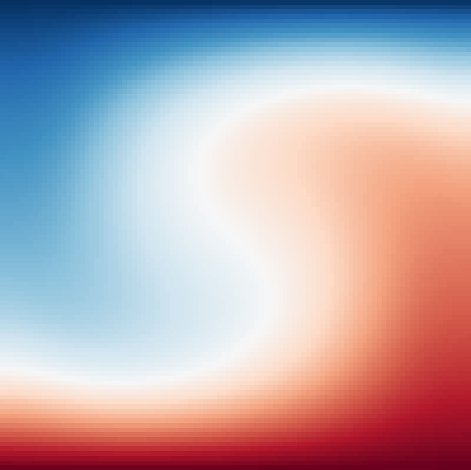
\includegraphics[width=\linewidth]{fig/rayleigh/T_no_control.png}} 
	\caption{Temperature}
\end{subfigure} \qquad
\begin{subfigure}[t]{.33\textwidth}
	\centering
	\fbox{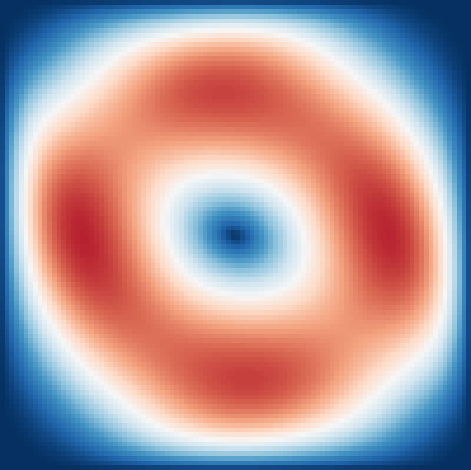
\includegraphics[width=\linewidth]{fig/rayleigh/u_no_control.png}} 
	\caption{Velocity norm}
\end{subfigure}
%%%%%%%%%%%%
\caption{\textbf{Temperature and velocity profiles for the Rayleigh-B\'enard convection cell} with $\ra=\num{1e4}$, $\pr=0.71$, $H=1$ and $L=1$.}
\label{fig:rayleigh_convection}
\end{figure}
%%%%%%%%%%%%
%%%%%%%%%%%%
%
%The situation is summed up in figure \ref{fig:sloshing_tank}. When excited laterally, the surface of the fluid sloshes back and forth in the tank generating complex patterns at the fluid surface, as shown in figure \ref{fig:sloshing_examples}. When the excitation stops, a relaxation phase is observed, usually leaving a single wavefront travelling back and forth in the tank until it dissipates entirely. Due to its simplicity, the model (\ref{eq:stvenant}) does not allow wave breaking nor the formation of drops on the sides of the domain.
%
%%%%%%%%%%%%%
%%%%%%%%%%%%
\begin{figure}
\centering
%%%%%%%%%%%%
\begin{tikzpicture}[]

	% ground
	\draw [thick] (-4,0) -- (4,0);

	% cart
	\draw [thick] (-2,0.5) -- (2,0.5);
	\draw [thick] (-2,0.5) -- (-2,2);
	\draw [thick] (2,0.5) -- (2,2);

	% wheels
	\draw [thick](-1.5,0.25) circle (0.25cm);
	\draw [thick] (1.5,0.25) circle (0.25cm);

	% water
	\begin{scope}
	    	\clip(-2,0.5) rectangle (2,2);
		\draw[draw=bluegray1,fill=cyan,fill opacity=0.5] plot [smooth cycle] coordinates {(-2.0,0.5+0.8) (-1.0,0.5+1.2) (0.0,0.5+1.0) (1.0,0.5+0.5) (2.0,0.5+0.9) (2.0,0.5+0.0) (-2.0,0.5+0.0)};
	\end{scope}

	% arrows and stuff
	\draw[-stealth] (-1.0,0.5) -- (-1.0,1.7) node[pos=0.5, anchor=west] {$h$};
	\draw[] (0,0.5) -- (0,1.5);
	\draw[-stealth] (0,1.0) -- (0.5,1.0) node[pos=0.5, anchor=north] {$q$};
	\draw[-stealth] (2.0,1.0) -- (3.0,1.0) node[pos=0.5, anchor=south] {$\ddot{y}$};
	
\end{tikzpicture}
%%%%%%%%%%%%
\caption{\textbf{Configuration of the sloshing tank.} The fluid flow is determined by the fluid height $h(x,t)$ and by its mass flow rate $q(x,t)$. The movement of the tank is controlled by its acceleration $\ddot{y}(t)$.} 
\label{fig:sloshing_tank}
\end{figure} 
%%%%%%%%%%%%
%%%%%%%%%%%%
%
%%%%%%%%%%%%%
%%%%%%%%%%%%
\begin{figure}
\centering
%%%%%%%%%%%%
%%%%%%%%%%%%
\begin{subfigure}{0.45\textwidth}
	\centering
	\begin{tikzpicture}[	scale=0.9, trim axis left, trim axis right, font=\scriptsize]
		\begin{axis}[	xmin=0, xmax=2.5, ymin=0, ymax=2, scale=1.0,
					xtick={0,0.5,1,1.5,2},
					width=\textwidth, height=.4\textwidth, scale only axis=true,
					legend cell align=left, legend pos=north east,
					grid=major, ylabel=$h$]
		
		\addplot[draw=bluegray1, very thick, smooth] 	table[x index=0,y index=1] {fig/sloshing/sloshing_excitation.dat};
			
		\end{axis}
	\end{tikzpicture}
    	\caption{Excitation phase}
	\label{fig:sloshing_excitation}
\end{subfigure} \quad
%%%%%%%%%%%%
\begin{subfigure}{0.45\textwidth}
	\centering
	\begin{tikzpicture}[	scale=0.9, trim axis left, trim axis right, font=\scriptsize]
		\begin{axis}[	xmin=0, xmax=2.5, ymin=0, ymax=2, scale=1.0,
					xtick={0,0.5,1,1.5,2},
					width=\textwidth, height=.4\textwidth, scale only axis=true,
					legend cell align=left, legend pos=north east,
					grid=major, ylabel={}]
		
			\addplot[draw=bluegray1, very thick, smooth] 	table[x index=0,y index=1] {fig/sloshing/sloshing_free.dat};
			
		\end{axis}
	\end{tikzpicture}
    	\caption{Relaxation phase}
	\label{fig:sloshing_free}
\end{subfigure}
%%%%%%%%%%%%
\caption{\textbf{Examples of fluid surface during the excitation phase (left) and the relaxation phase (right)}. The fluid height at rest is $h=1$.}
\label{fig:sloshing_examples}
\end{figure} 
%%%%%%%%%%%%
%%%%%%%%%%%%
%
%%%%%%%%%%%%%%%%%%%%%%%%%%%%%%%%%%%%%%%%%%%%%%%%%%%%%%%%%%
%%%%%%%%%%%%%%%%%%%%%%%%%%%%%%%%%%%%%%%%%%%%%%%%%%%%%%%%%%
%%%%%%%%%%%%%%%%%%%%%%%%%%%%%%%%%%%%%%%%%%%%%%%%%%%%%%%%%%
\section{Discretization}

The system (\ref{eq:rayleigh}) is discretized using a structured finite volume incremental projection scheme with centered fluxes, in the fashion of \cite{boivin2000}. For simplicity, the scheme is solved in a fully explicit way, except for the resolution of the Poisson equation for pressure. As is standard, a staggered grid is used for the finite volume scheme: the horizontal velocity is located on the west face of the cells, the vertical velocity is on the south face of the cells, while the pressure and temperature are located at the center of the cells. The computation of the instantaneous Nusselt number (\ref{eq:nusselt}) is performed by computing the first-order finite difference of the temperature between the center of the first cell at the bottom of the mesh and the reference temperature $T_H$. Doing so, we obtain $\nus = 2.16$  for $\ra = \num{1e4}$ once the permanent regime is reached, which is close to the reference values found in the literature, that range between $2.20$ and $2.24$ \cite{markatos1984}.

%%%%%%%%%%%%%%%%%%%%%%%%%%%%%%%%%%%%%%%%%%%%%%%%%%%%%%%%%%
%%%%%%%%%%%%%%%%%%%%%%%%%%%%%%%%%%%%%%%%%%%%%%%%%%%%%%%%%%
%%%%%%%%%%%%%%%%%%%%%%%%%%%%%%%%%%%%%%%%%%%%%%%%%%%%%%%%%%
\section{Environment}

The proposed environment is re-implemented based on the original publication of Beintema \textit{et al.} \cite{beintema2020}. In the following, we set $\pr=0.71$, which corresponds to the parameter for air, and $\ra = \num{1e4}$ in order to avoid high computational load. Similarly to \cite{beintema2020}, the control is performed by letting the DRL agent adjust the temperature of $n_s=10$ individual segments at the bottom of the cavity, the average temperature of the bottom plate being enforced to remain equal to $\theta_H$ (see figure \ref{fig:rayleigh_sketch_env}). To do so, the actions proposed by the agent are continuous temperature fluctuations $\left\{ \hat{\theta}_i \right\}_{i \in \llbracket 0, n_s-1 \rrbracket}$ in the range $\left[-C, +C\right]$, with $C=0.75$. To enforce $\left< \theta(y=0,x,t) \right> = \theta_H$, the provided $\hat{\theta}_i$ are normalized into the zero-average control $\theta_i$ as:

\begin{equation}
	\theta_i = \hat{\theta}_i - \left< \hat{\theta}_i \right>.
\end{equation}

For simplicity, no interpolation is performed between actions, neither spatially nor temporally. The spatial discretization step is set as $\Delta x = 0.02$, while the numerical time step is $\Delta t = 0.01$. The action time-step $\Delta t_\text{act}$ is equal to $1$ time unit, with the total episode length being fixed to $200$ time units, corresponding to $200$ actions.

%%%%%%%%%%%%
%%%%%%%%%%%%
\begin{figure}
\centering
\def\sc{0.6}
%%%%%%%%%%%%
\begin{tikzpicture}[	scale=\sc,
				probe/.style={circle, fill=gray1, inner sep=0pt, minimum size=2.5pt}]

	%%% large rectangle
	\draw[fill=white, draw=black, very thick] (-0.01,-1) rectangle (10.01,10);

	%%% picture
	\node[anchor=south west,inner sep=0, scale=\sc] (image) at (0,0) {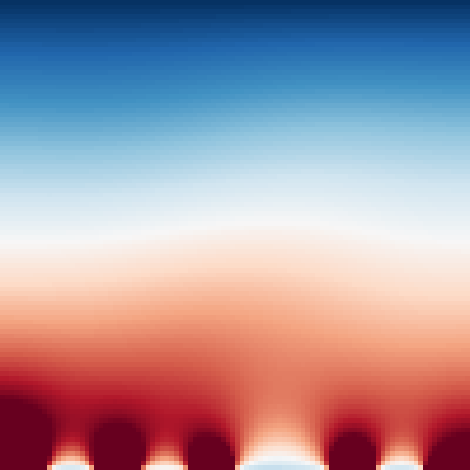
\includegraphics[width=9.99cm]{fig/rayleigh/T_control.png}};

	%%% probes
	\foreach \x in {0,...,7}
		\foreach \y in {0,...,7}
			\node[probe] at (0.5*1.25+1.25*\x,0.5*1.25+1.25*\y) {} ;
			
	%%% bottom frame
	\draw[fill=white] (0,-1) rectangle (10,0);
	\draw[dash pattern=on 2pt] (0,-0.5) -- (10, -0.5);
	\foreach \x in {1,...,9}
		\draw[dash pattern=on 1pt] (\x,-1) -- (\x,0);
		
	\draw[red, thick] (0,-0.5+0.5/0.75*0.75) -- (1, -0.5+0.5/0.75*0.75);
	\draw[blue, thick] (1,-0.5-0.5/0.75*0.42) -- (2, -0.5-0.5/0.75*0.42);
	\draw[blue,   thick] (2,-0.5-0.5/0.75*0.47) -- (3, -0.5-0.5/0.75*0.47);
	\draw[blue, thick] (3, -0.6) -- (4, -0.6);
	\draw[red, thick] (4,-0.2) -- (5, -0.2);
	\draw[red, thick] (5,-0.1) -- (6, -0.1);
	\draw[red, thick] (6,-0.3) -- (7, -0.3);
	\draw[blue, thick] (7,-0.7) -- (8, -0.7);
	\draw[blue, thick] (8,-0.9) -- (9, -0.9);
	\draw[blue, thick] (9,-0.6) -- (10, -0.6);

\end{tikzpicture}
%%%%%%%%%%%%
\caption{\textbf{Observation probes and actions imposition for the \codeinline{rayleigh-v0} environment}. The observations are collected at the probes regularly positioned in the domain, while the actions are imposed as piecewise-constant temperature boundary conditions on the bottom plate, with an average value equal to $\theta_H$.}
\label{fig:rayleigh_sketch_env}
\end{figure}
%%%%%%%%%%%%
%%%%%%%%%%%%

The observations provided to the agent are the temperatures collected on a grid of $n_p \times n_p$ probes evenly spaced in the computational domain (see figure \ref{fig:rayleigh_sketch_env}), along with the observations of the previous $n_h = 3$ time-steps. Contrarily to \cite{beintema2020}, the velocities are not provided to the agent. The resulting set of observations is flattened in a vector of size $(n_h+1) \times n_p^2$.

The reward at each times-step is simply set as the negative instantaneous Nusselt number, such that increasing the reward corresponds to a decrease of the temperature convection:

\begin{equation}
	r(t) = - \nus (t).
\end{equation}

Finally, each episode starts with the loading of a fully developed initial state obtained by solving the uncontrolled equations during a time $t_\text{init} = 200$ time units. The initial state corresponds to the field shown in figure \ref{fig:rayleigh_convection}. For convenience, this field is stored in a file and is loaded at the beginning of each episode. In case of modified parameters (spatial discretization, physical parameter...), this file can be generated by running the \codeinline{init.py} routine.

%%%%%%%%%%%%%%%%%%%%%%%%%%%%%%%%%%%%%%%%%%%%%%%%%%%%%%%%%%
%%%%%%%%%%%%%%%%%%%%%%%%%%%%%%%%%%%%%%%%%%%%%%%%%%%%%%%%%%
%%%%%%%%%%%%%%%%%%%%%%%%%%%%%%%%%%%%%%%%%%%%%%%%%%%%%%%%%%
\section{Results}

The environment as described in the previous section is referred to as \codeinline{rayleigh-v0}, and its default parameters are provided in table \ref{table:rayleigh_parameters}. In this section, we provide some results related to its resolution using a \textsc{ppo} agent (see the general hyperparameters in table \ref{table:default_ppo_parameters}). For the training, we set $n_\text{rollout} = 500$, $n_\text{batch} = 2$, $n_\text{epoch} = 32$ and $n_\text{max} = 200k$.
%
%The score curve obtained with the PPO algorithm is presented in \ref{fig:sloshing_score}, while the time evolutions of the controlled versus uncontrolled fluid level are shown in figure \ref{fig:sloshing_fields}. As can be observed, the agent manages to roughly cut the uncontrolled reward in half, by suppressing the back and forth wavefront using large actuations in the early stages of control, after what the control amplitude drops significantly.

%%%%%%%%%%%%
%%%%%%%%%%%%
\begin{table}
    \footnotesize
    \caption{\textbf{Default parameters used for the \codeinline{rayleigh-v0} environment.}}
    \label{table:rayleigh_parameters}
    \centering
    \begin{tabular}{rll}
        \toprule
        \codeinline{L}			& length of the domain					& $1$\\
	\codeinline{H}			& height of the domain					& $1$\\
	\codeinline{n_sgts}		& number of control segments				& $10$\\
	\codeinline{ra}			& Rayleigh number						& $\num{1e4}$\\
        \bottomrule
    \end{tabular}
\end{table}
%%%%%%%%%%%%
%%%%%%%%%%%%
%%
%%%%%%%%%%%%%
%%%%%%%%%%%%
\begin{figure}
\centering
%%%%%%%%%%%%
\begin{tikzpicture}[	trim axis left, trim axis right, font=\scriptsize,
				upper/.style={	name path=upper, smooth, draw=none},
				lower/.style={	name path=lower, smooth, draw=none},]
	\begin{axis}[	xmin=0, xmax=500000, scale=0.75,
				ymin=-6, ymax=0,
				scaled x ticks=false,
				xtick={0, 100000, 200000, 300000, 400000, 500000},
				xticklabels={$0$,$100k$,$200k$,$300k$,$400k$,$500k$},
				legend cell align=left, legend pos=south east,
				legend style={nodes={scale=0.8, transform shape}},
				every tick label/.append style={font=\scriptsize},
				grid=major, xlabel=transitions, ylabel=score]
				
		\legend{no control, \ppo, \ddpg}
		
		\addplot[thick, opacity=0.7, dash pattern=on 2pt]	coordinates {(0,-3.5) (500000,-3.5)};
		
		\addplot [upper, forget plot] 				table[x index=0,y index=7] {fig/burgers/ppo.dat};
		\addplot [lower, forget plot] 				table[x index=0,y index=6] {fig/burgers/ppo.dat}; 
		\addplot [fill=blue3, opacity=0.5, forget plot] 	fill between[of=upper and lower];
		\addplot[draw=blue1, thick, smooth] 			table[x index=0,y index=5] {fig/burgers/ppo.dat}; 
		
		\addplot [upper, forget plot] 				table[x index=0,y index=7] {fig/burgers/ddpg.dat};
		\addplot [lower, forget plot] 				table[x index=0,y index=6] {fig/burgers/ddpg.dat}; 
		\addplot [fill=green3, opacity=0.5, forget plot] 	fill between[of=upper and lower];
		\addplot[draw=green1, thick, smooth] 		table[x index=0,y index=5] {fig/burgers/ddpg.dat}; 
			
	\end{axis}
\end{tikzpicture}
%%%%%%%%%%%%
\caption{\textbf{Score curves for the \codeinline{burgers-v0} environment} solved with \ppo and \ddpg. The dashed line indicates the reward obtained for the uncontrolled environment.} 
\label{fig:burgers_score}
\end{figure} 
%%%%%%%%%%%%
%%%%%%%%%%%%
%%
%%%%%%%%%%%%%
%%%%%%%%%%%%
\begin{figure}
\centering
%%%%%%%%%%%%
\pgfdeclarelayer{background}
\pgfsetlayers{background,main}
%%%%%%%%%%%%
%%%%%%%%%%%%

\begin{subfigure}[t]{\textwidth}
	\centering
	\begin{tikzpicture}[	scale=0.7, trim axis left, trim axis right, font=\scriptsize]
		\begin{axis}[	xmin=0, xmax=270, ymin=0, ymax=2, scale=1.0,
					xtick={0,50,100,150,200,250,300},
					width=\textwidth, height=.15\textwidth, scale only axis=true,
					legend cell align=left, legend pos=north east,
					grid=major, ylabel=$h$]
				
		\def\x{150}
		\def\w{2}
		\def\s{10}

		\draw[fill=green2, draw=gray2] 			(\x+0*\s-\w,1) rectangle (\x+0*\s+\w,1+0.87);
		\draw[fill=green2, draw=gray2] 			(\x+1*\s-\w,1) rectangle (\x+1*\s+\w,1-0.35);
		\draw[fill=green2, draw=gray2] 			(\x+2*\s-\w,1) rectangle (\x+2*\s+\w,1+0.29);
		\draw[fill=green2, draw=gray2] 			(\x+3*\s-\w,1) rectangle (\x+3*\s+\w,1-0.29);
		\draw[fill=green2, draw=gray2] 			(\x+4*\s-\w,1) rectangle (\x+4*\s+\w,1-0.74);
		\draw[fill=green2, draw=gray2] 			(\x+5*\s-\w,1) rectangle (\x+5*\s+\w,1-0.88);
		\draw[fill=green2, draw=gray2] 			(\x+6*\s-\w,1) rectangle (\x+6*\s+\w,1-0.57);
		\draw[fill=green2, draw=gray2] 			(\x+7*\s-\w,1) rectangle (\x+7*\s+\w,1+0.62);
		\draw[fill=green2, draw=gray2] 			(\x+8*\s-\w,1) rectangle (\x+8*\s+\w,1+0.47);
		\draw[fill=green2, draw=gray2] 			(\x+9*\s-\w,1) rectangle (\x+9*\s+\w,1-0.47);
		
		\addplot[draw=gray1, very thick, smooth] 	table[x index=0,y index=1] {fig/shkadov/field_200.dat};
			
		\end{axis}
	\end{tikzpicture}
    	\caption{$t=200$, start of control}
	\label{fig:shkadov_fields_200}
\end{subfigure}

\medskip

%%%%%%%%%%%%
\begin{subfigure}[t]{\textwidth}
	\centering
	\begin{tikzpicture}[	scale=0.7, trim axis left, trim axis right, font=\scriptsize]
		\begin{axis}[	xmin=0, xmax=270, ymin=0, ymax=2, scale=1.0,
					xtick={0,50,100,150,200,250,300},
					width=\textwidth, height=.15\textwidth, scale only axis=true,
					legend cell align=left, legend pos=north east,
					grid=major, ylabel=$h$]
				
			\def\x{150}
			\def\w{2}
			\def\s{10}
		
			\draw[fill=green2, draw=gray2] 			(\x+0*\s-\w,1) rectangle (\x+0*\s+\w,1+0.22);
			\draw[fill=green2, draw=gray2] 			(\x+1*\s-\w,1) rectangle (\x+1*\s+\w,1-0.13);
			\draw[fill=green2, draw=gray2] 			(\x+2*\s-\w,1) rectangle (\x+2*\s+\w,1-0.17);
			\draw[fill=green2, draw=gray2] 			(\x+3*\s-\w,1) rectangle (\x+3*\s+\w,1+0.077);
			\draw[fill=green2, draw=gray2] 			(\x+4*\s-\w,1) rectangle (\x+4*\s+\w,1+0.039);
			\draw[fill=green2, draw=gray2] 			(\x+5*\s-\w,1) rectangle (\x+5*\s+\w,1+0.045);
			\draw[fill=green2, draw=gray2] 			(\x+6*\s-\w,1) rectangle (\x+6*\s+\w,1-0.033);
			\draw[fill=green2, draw=gray2] 			(\x+7*\s-\w,1) rectangle (\x+7*\s+\w,1+0.095);
			\draw[fill=green2, draw=gray2] 			(\x+8*\s-\w,1) rectangle (\x+8*\s+\w,1-0.17);
			\draw[fill=green2, draw=gray2] 			(\x+9*\s-\w,1) rectangle (\x+9*\s+\w,1-0.12);
		
			\addplot[draw=gray1, very thick, smooth] 	table[x index=0,y index=1] {fig/shkadov/field_300.dat};
			
		\end{axis}
	\end{tikzpicture}
    	\caption{$t=300$}
	\label{fig:shkadov_fields_300}
\end{subfigure}

\medskip

%%%%%%%%%%%%
\begin{subfigure}[t]{\textwidth}
	\centering
	\begin{tikzpicture}[	scale=0.7, trim axis left, trim axis right, font=\scriptsize]
		\begin{axis}[	xmin=0, xmax=270, ymin=0, ymax=2, scale=1.0,
					xtick={0,50,100,150,200,250,300},
					width=\textwidth, height=.15\textwidth, scale only axis=true,
					legend cell align=left, legend pos=north east,
					grid=major, ylabel=$h$]
				
			\def\x{150}
			\def\w{2}
			\def\s{10}
		
			\draw[fill=green2, draw=gray2] 			(\x+0*\s-\w,1) rectangle (\x+0*\s+\w,1+0.12);
			\draw[fill=green2, draw=gray2] 			(\x+1*\s-\w,1) rectangle (\x+1*\s+\w,1+0.027);
			\draw[fill=green2, draw=gray2] 			(\x+2*\s-\w,1) rectangle (\x+2*\s+\w,1-0.22);
			\draw[fill=green2, draw=gray2] 			(\x+3*\s-\w,1) rectangle (\x+3*\s+\w,1+0.015);
			\draw[fill=green2, draw=gray2] 			(\x+4*\s-\w,1) rectangle (\x+4*\s+\w,1+0.065);
			\draw[fill=green2, draw=gray2] 			(\x+5*\s-\w,1) rectangle (\x+5*\s+\w,1-0.027);
			\draw[fill=green2, draw=gray2] 			(\x+6*\s-\w,1) rectangle (\x+6*\s+\w,1+0.0049);
			\draw[fill=green2, draw=gray2] 			(\x+7*\s-\w,1) rectangle (\x+7*\s+\w,1+0.0070);
			\draw[fill=green2, draw=gray2] 			(\x+8*\s-\w,1) rectangle (\x+8*\s+\w,1-0.12);
			\draw[fill=green2, draw=gray2] 			(\x+9*\s-\w,1) rectangle (\x+9*\s+\w,1-0.0091);
		
			\addplot[draw=gray1, very thick, smooth] 	table[x index=0,y index=1] {fig/shkadov/field_400.dat};
			
		\end{axis}
	\end{tikzpicture}
    	\caption{$t=400$}
	\label{fig:shkadov_fields_300}
\end{subfigure}

\medskip

%%%%%%%%%%%%
\begin{subfigure}[t]{\textwidth}
	\centering
	\begin{tikzpicture}[	scale=0.7, trim axis left, trim axis right, font=\scriptsize]
		\begin{axis}[	xmin=0, xmax=270, ymin=0, ymax=2, scale=1.0,
					xtick={0,50,100,150,200,250,300},
					width=\textwidth, height=.15\textwidth, scale only axis=true,
					legend cell align=left, legend pos=north east,
					grid=major, ylabel=$h$]
				
			\def\x{150}
			\def\w{2}
			\def\s{10}
		
			\draw[fill=green2, draw=gray2] 			(\x+0*\s-\w,1) rectangle (\x+0*\s+\w,1+0.098);
			\draw[fill=green2, draw=gray2] 			(\x+1*\s-\w,1) rectangle (\x+1*\s+\w,1+0.095);
			\draw[fill=green2, draw=gray2] 			(\x+2*\s-\w,1) rectangle (\x+2*\s+\w,1-0.18);
			\draw[fill=green2, draw=gray2] 			(\x+3*\s-\w,1) rectangle (\x+3*\s+\w,1-0.011);
			\draw[fill=green2, draw=gray2] 			(\x+4*\s-\w,1) rectangle (\x+4*\s+\w,1+0.083);
			\draw[fill=green2, draw=gray2] 			(\x+5*\s-\w,1) rectangle (\x+5*\s+\w,1-0.026);
			\draw[fill=green2, draw=gray2] 			(\x+6*\s-\w,1) rectangle (\x+6*\s+\w,1+0.010);
			\draw[fill=green2, draw=gray2] 			(\x+7*\s-\w,1) rectangle (\x+7*\s+\w,1+0.025);
			\draw[fill=green2, draw=gray2] 			(\x+8*\s-\w,1) rectangle (\x+8*\s+\w,1-0.12);
			\draw[fill=green2, draw=gray2] 			(\x+9*\s-\w,1) rectangle (\x+9*\s+\w,1-0.032);
		
			\addplot[draw=gray1, very thick, smooth] 	table[x index=0,y index=1] {fig/shkadov/field_500.dat};
			
		\end{axis}
	\end{tikzpicture}
    	\caption{$t=500$}
	\label{fig:shkadov_fields_500}
\end{subfigure}

\medskip

%%%%%%%%%%%%
\begin{subfigure}[t]{\textwidth}
	\centering
	\begin{tikzpicture}[	scale=0.7, trim axis left, trim axis right, font=\scriptsize]
		\begin{axis}[	xmin=0, xmax=270, ymin=0, ymax=2, scale=1.0,
					xtick={0,50,100,150,200,250,300},
					width=\textwidth, height=.15\textwidth, scale only axis=true,
					legend cell align=left, legend pos=north east,
					grid=major, ylabel=$h$]
				
			\def\x{150}
			\def\w{2}
			\def\s{10}
		
			\draw[fill=green2, draw=gray2] 			(\x+0*\s-\w,1) rectangle (\x+0*\s+\w,1+0.16);
			\draw[fill=green2, draw=gray2] 			(\x+1*\s-\w,1) rectangle (\x+1*\s+\w,1+0.042);
			\draw[fill=green2, draw=gray2] 			(\x+2*\s-\w,1) rectangle (\x+2*\s+\w,1-0.15);
			\draw[fill=green2, draw=gray2] 			(\x+3*\s-\w,1) rectangle (\x+3*\s+\w,1+0.031);
			\draw[fill=green2, draw=gray2] 			(\x+4*\s-\w,1) rectangle (\x+4*\s+\w,1+0.042);
			\draw[fill=green2, draw=gray2] 			(\x+5*\s-\w,1) rectangle (\x+5*\s+\w,1-0.058);
			\draw[fill=green2, draw=gray2] 			(\x+6*\s-\w,1) rectangle (\x+6*\s+\w,1-0.028);
			\draw[fill=green2, draw=gray2] 			(\x+7*\s-\w,1) rectangle (\x+7*\s+\w,1+0.058);
			\draw[fill=green2, draw=gray2] 			(\x+8*\s-\w,1) rectangle (\x+8*\s+\w,1-0.095);
			\draw[fill=green2, draw=gray2] 			(\x+9*\s-\w,1) rectangle (\x+9*\s+\w,1-0.014);
		
			\addplot[draw=gray1, very thick, smooth] 	table[x index=0,y index=1] {fig/shkadov/field_600.dat};
			
		\end{axis}
	\end{tikzpicture}
    	\caption{$t=600$}
	\label{fig:shkadov_fields_600}
\end{subfigure}

\medskip

%%%%%%%%%%%%
\begin{subfigure}[t]{\textwidth}
	\centering
	\begin{tikzpicture}[	scale=0.7, trim axis left, trim axis right, font=\scriptsize]
		\begin{axis}[	xmin=0, xmax=270, ymin=0, ymax=2, scale=1.0,
					xtick={0,50,100,150,200,250,300},
					width=\textwidth, height=.15\textwidth, scale only axis=true,
					legend cell align=left, legend pos=north east,
					grid=major, ylabel=$h$]
				
			\def\x{150}
			\def\w{2}
			\def\s{10}
		
			\draw[fill=green2, draw=gray2] 			(\x+0*\s-\w,1) rectangle (\x+0*\s+\w,1+0.21);
			\draw[fill=green2, draw=gray2] 			(\x+1*\s-\w,1) rectangle (\x+1*\s+\w,1+0.021);
			\draw[fill=green2, draw=gray2] 			(\x+2*\s-\w,1) rectangle (\x+2*\s+\w,1-0.15);
			\draw[fill=green2, draw=gray2] 			(\x+3*\s-\w,1) rectangle (\x+3*\s+\w,1+0.048);
			\draw[fill=green2, draw=gray2] 			(\x+4*\s-\w,1) rectangle (\x+4*\s+\w,1+0.044);
			\draw[fill=green2, draw=gray2] 			(\x+5*\s-\w,1) rectangle (\x+5*\s+\w,1-0.071);
			\draw[fill=green2, draw=gray2] 			(\x+6*\s-\w,1) rectangle (\x+6*\s+\w,1-0.038);
			\draw[fill=green2, draw=gray2] 			(\x+7*\s-\w,1) rectangle (\x+7*\s+\w,1+0.034);
			\draw[fill=green2, draw=gray2] 			(\x+8*\s-\w,1) rectangle (\x+8*\s+\w,1-0.093);
			\draw[fill=green2, draw=gray2] 			(\x+9*\s-\w,1) rectangle (\x+9*\s+\w,1-0.046);
		
			\addplot[draw=gray1, very thick, smooth] 	table[x index=0,y index=1] {fig/shkadov/field_700.dat};
			
		\end{axis}
	\end{tikzpicture}
    	\caption{$t=700$}
	\label{fig:shkadov_fields_700}
\end{subfigure}
%%%%%%%%%%%%
\caption{\textbf{Evolution of the flow under control of the agent, using 10 jets.} The jets strengths are represented with green rectangles.}
\label{fig:shkadov_fields}
\end{figure} 
%%%%%%%%%%%%
%%%%%%%%%%%%
